\documentclass[12pt,letterpaper]{article}

% Idioma y codificación
\usepackage[spanish]{babel}
\usepackage[utf8]{inputenc}
\usepackage[T1]{fontenc}

% Márgenes y formato
\usepackage{geometry}
\geometry{
    left=2.5cm,
    right=2.5cm,
    top=2.5cm,
    bottom=2.5cm
}

% Imágenes, tablas y colores
\usepackage{graphicx}
\usepackage{float}
\usepackage{array}
\usepackage{booktabs}
\usepackage{xcolor}
\usepackage{caption}
\usepackage{ragged2e}
\usepackage{microtype}

% Encabezado y pie de página
\usepackage{fancyhdr}

% Fuente parecida a Word
\usepackage{helvet}
\renewcommand{\familydefault}{\sfdefault}

% Espaciado
\usepackage{setspace}
\setstretch{1.0}

% Justificación y párrafos estilo Word
\setlength{\parindent}{0pt}
\setlength{\parskip}{0.6em}

\renewcommand{\theenumi}{\roman{enumi}}
\renewcommand{\labelenumi}{\theenumi.}

% Hipervínculos
\usepackage{hyperref}

% Color similar al azul de títulos
\definecolor{unalblue}{RGB}{31,78,121}

% Formato de títulos
\usepackage{titlesec}

\titleformat{\section}
  {\normalfont\large\bfseries\color{unalblue}}
  {\thesection.}
  {0.5em}
  {}

\titleformat{\subsection}
  {\normalfont\normalsize\bfseries}
  {\thesubsection}
  {0.5em}
  {}

% Encabezado con logo
\pagestyle{fancy}
\fancyhf{}
\fancyhead[R]{
\includegraphics[width=3cm]{logo_unal.png}}
\renewcommand{\headrulewidth}{0pt}
\fancyfoot[C]{\thepage}

% Figuras
\captionsetup{
    font=small,
    labelfont=bf,
    justification=centering
}

\begin{document}

{
\begin{titlepage}
    \centering

    % Logo en la parte superior derecha
    \begin{flushright}
        
\includegraphics[width=3cm]{logo_unal.png}
    \end{flushright}

    \vspace{0.5cm}

    {\small \textbf{ESPECIALIZACIÓN EN INTELIGENCIA ARTIFICIAL}\par}

    \vspace{3.8cm}

    {\small PROYECTO FINAL BUSINESS ANALYTICS\par}

    \vspace{0.3cm}

    {\small \underline{\textbf{Implementación de un Data Warehouse}}\par}

    \vspace{3.8cm}

    {\small \textbf{Elaborado por:}\par}
    {\small SERGIO ALEJANDRO VILLADA ARIAS\par}
    {\small JULIÁN DAVID ARANZAZU VELÁSQUEZ\par}

    \vspace{3cm}

    {\small \textbf{Docente:}\par}
    {\small LUZ ENITH GUERRERO MENDIETA\par}

    \vfill

    {\small \textbf{Facultad de Administración}\par}
    {\small \textbf{Universidad Nacional de Colombia}\par}
    {\small \textbf{Manizales, Colombia}\par}

\end{titlepage}
}

\newpage

\justifying
\section*{Descripción del Problema}

\subsection*{Contexto del Problema}

\noindent En la actualidad, uno de los mayores desafíos a nivel global es comprender cómo las variaciones climáticas impactan directamente en la seguridad alimentaria y, en consecuencia, en la economía mundial. Eventos como sequías prolongadas o picos históricos de temperatura no solo afectan la cantidad de alimentos que se pueden cosechar en un país, sino que también generan escasez, lo que inevitablemente dispara los precios de los productos en el mercado internacional.

\noindent Para poder medir, cruzar y analizar este fenómeno desde una perspectiva de Business Analytics, hemos formulado un proyecto que busca encontrar la relación directa entre el clima, la producción agrícola y los precios del mercado. Para lograrlo, integramos la información de tres fuentes de datos públicas, heterogéneas y de alta fiabilidad:

\begin{enumerate}
    \item \textbf{Berkeley Earth:} Es una base de datos científica independiente que registra las temperaturas de la superficie terrestre. De aquí extrajimos los registros históricos de las anomalías térmicas (es decir, qué tanto más calor o frío hizo frente a lo normal) medidos de forma mensual y detallados por país. Esta es nuestra principal fuente para entender el comportamiento climático.
    \item \textbf{FAOSTAT:} Es la base de datos oficial de la Organización de las Naciones Unidas para la Alimentación y la Agricultura (FAO). Esta fuente nos proporciona las métricas exactas sobre el sector agropecuario a nivel mundial. De aquí tomamos los datos de volumen de producción, rendimiento de la tierra y áreas cosechadas para cultivos clave, organizados por año y por país.
    \item \textbf{Pinky Rose FIM (Fondo Monetario Internacional / Precios de Commodities):} Para conectar el clima y la agricultura con el impacto financiero, utilizamos esta fuente que rastrea el valor de los productos básicos (commodities) en los mercados globales. Nos aporta el precio de cotización mensual de diferentes rubros agrícolas. A diferencia de las otras dos fuentes, estos precios son un estándar global, lo que nos permite evaluar cómo un problema de cosecha en regiones clave afecta el bolsillo a nivel mundial.
\end{enumerate}

\noindent Al integrar estas tres fuentes (que originalmente están en formatos y estructuras diferentes), el proyecto busca romper los silos de información. La idea no es solo mirar un reporte del clima o un reporte de finanzas por separado, sino construir un Data Warehouse que nos permita ver la "película completa" y respaldar la toma de decisiones basada en la evidencia de los datos.
\subsection*{Objetivos analíticos}

\noindent El objetivo general de este proyecto es diseñar e implementar una solución de  Business Analytics, apoyada en un Data Warehouse, que permita comprender cómo las variaciones climáticas pueden afectar de manera directa la producción agrícola y, a partir de eso, influir también en los precios de los productos en el mercado global. La idea es integrar información de clima, agricultura y economía para analizar de forma conjunta estos tres componentes y así tener una visión más completa del problema, especialmente en temas relacionados con seguridad alimentaria y comportamiento de precios.

\noindent Para lograrlo, primero se busca extraer, limpiar e integrar los datos históricos provenientes de Berkeley Earth, FAOSTAT y Pinky Rose FIM, de manera que toda la información quede reunida en un solo repositorio y se elimine el manejo aislado de las fuentes. Después, se plantea construir un modelo de datos que permita relacionar las variables climáticas, agrícolas y económicas a partir de elementos comunes como el año, el mes y el país. 

\noindent Con esta base, también se espera desarrollar tableros de control que faciliten la visualización del comportamiento de los datos y permitan identificar de forma más clara si los periodos de anomalías climáticas, como excesos de calor o frío, coinciden con disminuciones en la producción agrícola y aumentos en los precios de los alimentos. Finalmente, se propone incorporar herramientas de inteligencia artificial sobre los datos ya integrados, con el fin de apoyar la interpretación de los resultados, encontrar patrones que no sean tan evidentes a simple vista y darle un valor agregado al análisis realizado de forma tradicional.

\subsection*{Justificación de Valor}

\noindent El valor fundamental de este proyecto radica en su capacidad para transformar datos históricos y dispersos en conocimiento accionable para la toma de decisiones estratégicas. Tradicionalmente, el análisis del impacto climático sobre la agricultura y la economía se hace de manera reactiva y fragmentada, pero al centralizar estas tres fuentes en un Data Warehouse creamos una "única fuente de verdad" que permite cruzar las variables de forma natural. El verdadero diferencial no es solo visualizar lo que ya pasó, sino preparar el terreno para que las herramientas de Inteligencia Artificial descubran patrones ocultos —como identificar cuánto tiempo tarda una anomalía térmica en encarecer un commodity específico—. Esto proporciona a investigadores, analistas o responsables de políticas públicas una base sólida y fundamentada en evidencia empírica para anticipar escenarios, formular estrategias de seguridad alimentaria o tomar decisiones de mercado, pasando de la intuición a una gestión verdaderamente basada en datos para tomar decisiones de mercado.

\noindent acuerdo con lo expuesto a manera de antesala del proyecto, a continuación, se desarrollarán las 6 fases del proyecto.
\newpage
\section{Parte 1. Procesos de Extracción, Transformación y Carga - ETL}

\noindent Como parte de la \underline{descripción del proceso seguido}, y como se ha mencionado anteriormente, fueron utilizadas tres fuentes de datos (Berkeleyn Earth, FAOSTAT, Pinky Rose FIM), de las cuales los datos se encontraban dispersos, con diferencias en su estructura, inconsistencias en su presentación, dificultades en la calidad, entre otros.

\noindent Por parte de \textbf{Berkeley Earth}, fueron obtenidos 164 archivos .txt con información climática correspondiente a 164 países. Al analizar la estructura interna de estos documentos, tomando como caso de estudio el archivo united-states.txt (Estados Unidos), identificamos las siguientes características y retos para su procesamiento
\begin{itemize}
    \item \textbf{Metadatos integrados:} El archivo no inicia directamente con la tabla de datos, sino con un extenso encabezado de texto (comentado con el símbolo \%). Este bloque explica la metodología de medición, indicando que las temperaturas están en grados Celsius y se reportan como anomalías en relación con el promedio histórico del periodo 1951-1980 (para el caso de Estados Unidos). En el proceso ETL, este encabezado debió ser filtrado para poder leer la matriz de datos.
    \item \textbf{Estructura del archivo:} Los datos no están separados por comas (como en un CSV tradicional), sino por espacios en blanco tabulados. La tabla contiene múltiples columnas, de las cuales identificamos como críticas para nuestro modelo: el Año (Year), el Mes (Month), la Anomalía Mensual (Monthly Anomaly) y la Incertidumbre Mensual (Monthly Uncertainty).
    \item \textbf{Problemas de Calidad (Datos Nulos):} El archivo presenta una gran cantidad de datos faltantes registrados bajo la etiqueta NaN (Not a Number), especialmente en los registros históricos más antiguos y en las columnas de promedios suavizados (a 1, 5 o 10 años). Por ello se hizo necesario establecer un rango de tiempo dónde se analizarán los datos, se tomó como punto de partida el año 1990 dónde empiezan los reportes del Pinky Rose y como año de finalización se tomó el año 2015 que es el último reporte de esta base de datos, de esta manera nos eliminamos el problema de los datos etiquetados con NaN.
    
    \begin{figure}[H]
    	\centering
    	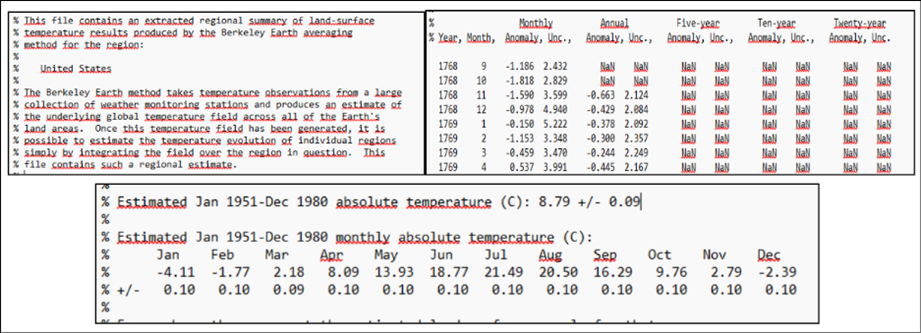
\includegraphics[width=0.8\linewidth]{estructure_berkeley_example.png}
    	\caption{Estructura original del archivo de Berkeley Earth.}
    	\label{fig:berkeley-structure}
    	
    	\vspace{0.2cm}
    	\footnotesize Fuente: Elaboración propia con base en datos de Berkeley Earth.
    \end{figure}
    Para convertir estos datos planos en una tabla estructurada, y poder analizar la información asertivamente, fueron desarrollados los siguientes scripts en Python que denominamos \textbf{01\_country\_name\_mapping.py}, \textbf{02\_download\_berkeley\_files.py} y \textbf{03\_transform\_berkeley\_txt.py} (Scripts ETL), los cuales se encargaron de automatizar la extracción, estructurar el contenido y resolver problemas de calidad de datos: 
\end{itemize}

\newpage
%\input{sections/03_modelamiento}

\newpage
%\input{sections/04_implementacion}

\newpage
%\input{sections/05_visualizacion}

\newpage
%\input{sections/06_explotacion}

\newpage
%\input{sections/07_integracion_ia}

\newpage
%\input{sections/02_etl}

\newpage
%\input{sections/03_modelamiento}

\newpage
%\input{sections/04_implementacion}

\newpage
%\input{sections/05_visualizacion}

\newpage
%\input{sections/06_explotacion}

\newpage
%\input{sections/07_integracion_ia}

\end{document}
